\chapter{Estado del arte}
La introducción original de la idea de modelar usando superficies implícitas fue hecha por Jim Blinn en 1982, en un artículo \cite{blinn1982generalization} donde presenta un método para representar superficies dadas por ecuaciones de orden mayor a dos usando funciones de densidad Gaussianas. Este modelo tenía la ventaja de permitir la combinación suave de primitivas, y en los siguientes años surgirían modelos similares tratando de conseguir esto mismo bajo la denominación de \textit{Blobby Molecules}, debido a la capacidad que tienen estos de combinar primitivas. Entre ellos destaca el de A. Pasko en 1995 \cite{pasko1995function}, que era más completo que el de Blinn al incluir la posibilidad de aplicar operadores de deformación y booleanos. Llegado 1999, Brian Wyvill, Eric Galin y Andrew Guy presentan en su artículo \textit{The BlobTree: Warping, Blending and Boolean Operations in an Implicit Surface Modeling System} \cite{blobtree} el modelo \textit{BlobTree}, que permite realizar las mismas funciones que los modelos anteriores de forma más estructurada, y motiva el desarrollo de este trabajo.\newline

Las ventajas que aporta el uso de funciones distancia con signo hace que podamos ver su uso en multitud de productos actuales, entre los que destacamos los siguientes.
\begin{itemize}
    \item A través de un algoritmo que permite obtener la representación por SDF de una malla de triángulos, Blender \cite{repo:blender} utiliza SDFs para realizar geometría de sólidos constructiva y otras operaciones de cuerpo blando.
    \item Clayxels \cite{clayxels} es un paquete para el motor Unity3D que permite esculpir modelos combinando primitivas definidas por SDFs y convertir el resultado a una malla de polígonos que pueda ser usada de forma convencional en el motor.
    \item El motor Unreal Engine \cite{unreal} incorpora una funcionalidad para aproximar la función distancia con signo de los modelos estáticos en escena y almacenar dicha información en una textura. Una vez realizado este proceso, usa los datos para cálculos de sombras y oclusión ambiental dinámica. También permite usar la SDF para calcular colisiones de partículas (Unity3D también tiene esta característica), calcular mapas de flujo, etc.   
    \item Claybook \cite{claybook} es un videojuego que implementa un escenario totalmente destructible definido mediante SDFs y renderizado con \textit{raytracing}. Utiliza varias de las técnicas de renderizado que veremos en el \autoref{cap:2}.
    \item Dreams \cite{game:dreams} es un videojuego que permite a los jugadores crear y programar nuevas experiencias interactivas que compartir con los usuarios. Entre sus funcionalidades se incluye la creación de modelos 3D en tiempo real, que usa operadores booleanos suavizados sobre funciones distancia con signo de forma interna y transparente al jugador.
\end{itemize}
\begin{figure}[!h]
    \centering
    \begin{subfigure}[b]{0.45\textwidth}
        \centering
        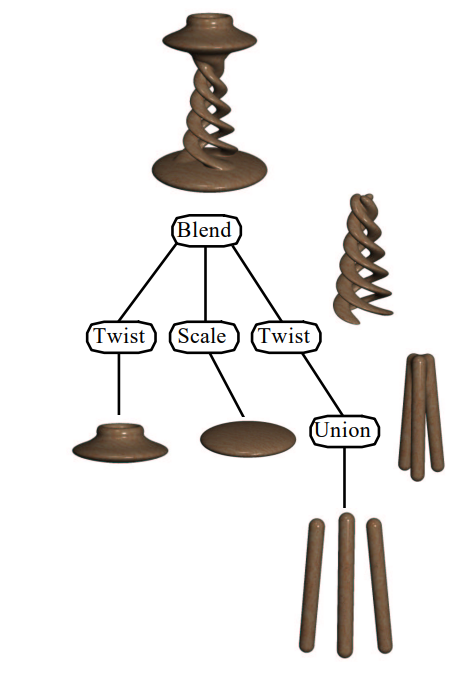
\includegraphics[width=\textwidth]{Plantilla-TFG-master/img/blobtree.png}
        \caption{Ejemplo de uso del modelo \textit{BlobTree} \cite{blinn1982generalization} }
    \end{subfigure}
    \hspace{15pt}
    \begin{subfigure}[b]{0.45\textwidth}
        \centering
        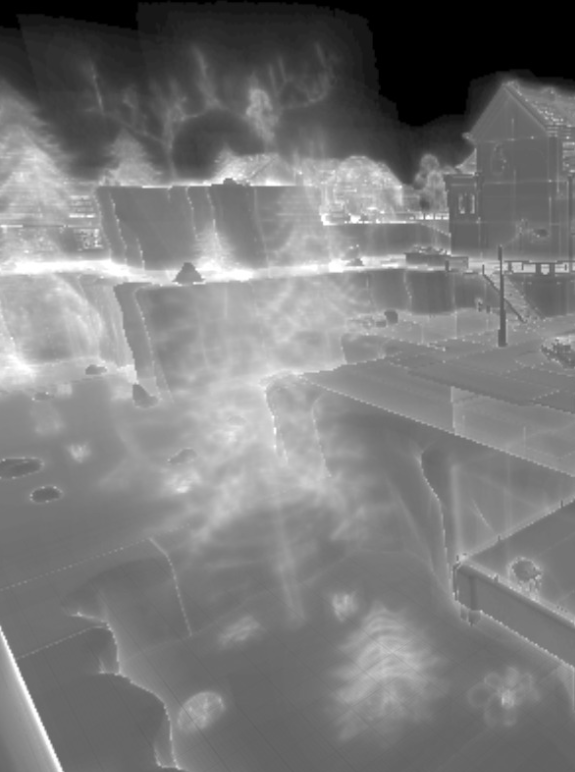
\includegraphics[width=\textwidth]{Plantilla-TFG-master/img/sdf_unreal.png}
        \caption{Visualización de la SDF de una escena en Unreal Engine \cite{unreal}}
    \end{subfigure}
    \hfill
\end{figure}


No podemos dejar de mencionar la contribución del español Íñigo Quílez. Su blog \cite{Quilez_undated-oh} contiene artículos relacionados con la IG y las matemáticas usadas en ella, y su sección dedicada a las SDFs y el \textit{raymarching} ha sido una inspiración a lo largo del desarrollo de este trabajo. Esta incluye artículos que discuten varios de los temas aquí tratados, como la oclusión ambiental, cálculo de normales, etc., e incluye una lista muy útil de primitivas y operadores de SDFs. Además de esta contribución teórica, Íñigo Quílez es también el coautor junto a Pol Jeremías de ShaderToy \cite{shadertoy}, una plataforma en la que crear y compartir obras generadas con un \textit{fragment shader} sobre un lienzo. En ella hay muchos ejemplos de uso de técnicas avanzadas sobre SDFs con \textit{raytracing} (\autoref{fig:shadertoy}), similares a las que desarrollaremos en profundidad en los siguientes capítulos.
\begin{figure}[!h]
    \centering
    \begin{subfigure}[b]{0.45\textwidth}
        \centering
        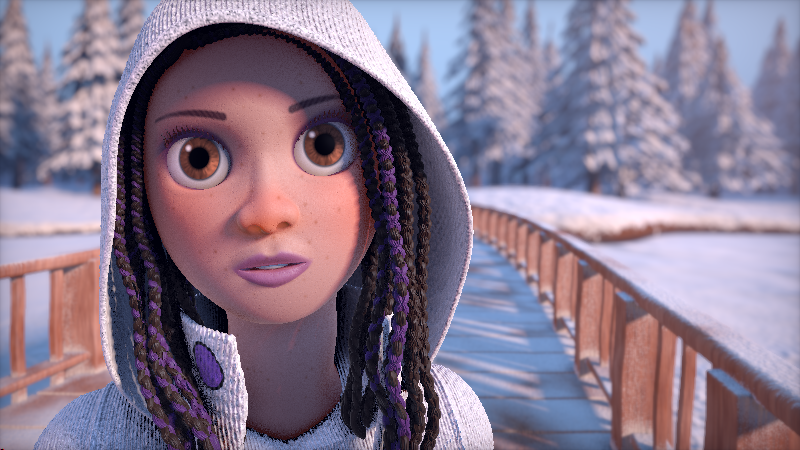
\includegraphics[width=\textwidth]{Plantilla-TFG-master/img/shadertoy1.png}
        \caption{\qq{\textit{Selfie Girl}} \cite{shader2}, Íñigo Quílez}
    \end{subfigure}
    \hspace{15pt}
    \begin{subfigure}[b]{0.45\textwidth}
        \centering
        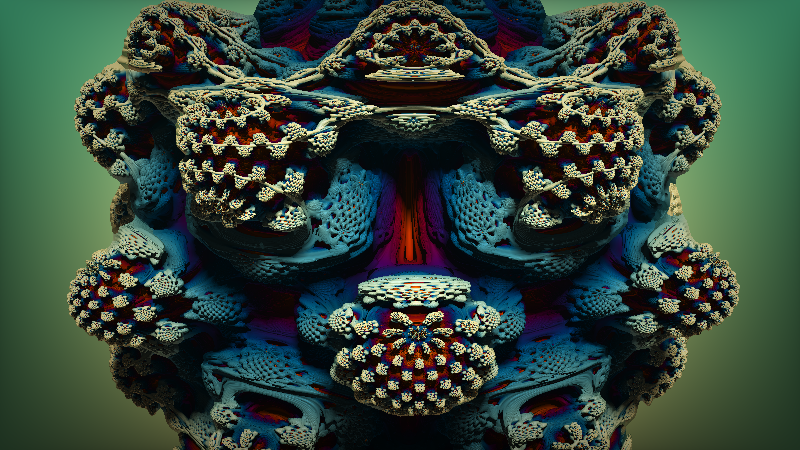
\includegraphics[width=\textwidth]{Plantilla-TFG-master/img/shadertoy2.png}
        \caption{Mandelbulbo \cite{shader1}, usuario EvilRyu}
    \end{subfigure}
    \hfill
     \caption{Ejemplos de obras creadas en Shadertoy usando únicamente SDFs}
     \label{fig:shadertoy}
\end{figure}
